% Options for packages loaded elsewhere
\PassOptionsToPackage{unicode}{hyperref}
\PassOptionsToPackage{hyphens}{url}
%
\documentclass[
]{article}
\usepackage{lmodern}
\usepackage{amssymb,amsmath}
\usepackage{ifxetex,ifluatex}
\ifnum 0\ifxetex 1\fi\ifluatex 1\fi=0 % if pdftex
  \usepackage[T1]{fontenc}
  \usepackage[utf8]{inputenc}
  \usepackage{textcomp} % provide euro and other symbols
\else % if luatex or xetex
  \usepackage{unicode-math}
  \defaultfontfeatures{Scale=MatchLowercase}
  \defaultfontfeatures[\rmfamily]{Ligatures=TeX,Scale=1}
\fi
% Use upquote if available, for straight quotes in verbatim environments
\IfFileExists{upquote.sty}{\usepackage{upquote}}{}
\IfFileExists{microtype.sty}{% use microtype if available
  \usepackage[]{microtype}
  \UseMicrotypeSet[protrusion]{basicmath} % disable protrusion for tt fonts
}{}
\makeatletter
\@ifundefined{KOMAClassName}{% if non-KOMA class
  \IfFileExists{parskip.sty}{%
    \usepackage{parskip}
  }{% else
    \setlength{\parindent}{0pt}
    \setlength{\parskip}{6pt plus 2pt minus 1pt}}
}{% if KOMA class
  \KOMAoptions{parskip=half}}
\makeatother
\usepackage{xcolor}
\IfFileExists{xurl.sty}{\usepackage{xurl}}{} % add URL line breaks if available
\IfFileExists{bookmark.sty}{\usepackage{bookmark}}{\usepackage{hyperref}}
\hypersetup{
  pdftitle={Fitbit Data Analysis},
  pdfauthor={Marie-Luise Fischer},
  hidelinks,
  pdfcreator={LaTeX via pandoc}}
\urlstyle{same} % disable monospaced font for URLs
\usepackage[margin=1in]{geometry}
\usepackage{color}
\usepackage{fancyvrb}
\newcommand{\VerbBar}{|}
\newcommand{\VERB}{\Verb[commandchars=\\\{\}]}
\DefineVerbatimEnvironment{Highlighting}{Verbatim}{commandchars=\\\{\}}
% Add ',fontsize=\small' for more characters per line
\usepackage{framed}
\definecolor{shadecolor}{RGB}{248,248,248}
\newenvironment{Shaded}{\begin{snugshade}}{\end{snugshade}}
\newcommand{\AlertTok}[1]{\textcolor[rgb]{0.94,0.16,0.16}{#1}}
\newcommand{\AnnotationTok}[1]{\textcolor[rgb]{0.56,0.35,0.01}{\textbf{\textit{#1}}}}
\newcommand{\AttributeTok}[1]{\textcolor[rgb]{0.77,0.63,0.00}{#1}}
\newcommand{\BaseNTok}[1]{\textcolor[rgb]{0.00,0.00,0.81}{#1}}
\newcommand{\BuiltInTok}[1]{#1}
\newcommand{\CharTok}[1]{\textcolor[rgb]{0.31,0.60,0.02}{#1}}
\newcommand{\CommentTok}[1]{\textcolor[rgb]{0.56,0.35,0.01}{\textit{#1}}}
\newcommand{\CommentVarTok}[1]{\textcolor[rgb]{0.56,0.35,0.01}{\textbf{\textit{#1}}}}
\newcommand{\ConstantTok}[1]{\textcolor[rgb]{0.00,0.00,0.00}{#1}}
\newcommand{\ControlFlowTok}[1]{\textcolor[rgb]{0.13,0.29,0.53}{\textbf{#1}}}
\newcommand{\DataTypeTok}[1]{\textcolor[rgb]{0.13,0.29,0.53}{#1}}
\newcommand{\DecValTok}[1]{\textcolor[rgb]{0.00,0.00,0.81}{#1}}
\newcommand{\DocumentationTok}[1]{\textcolor[rgb]{0.56,0.35,0.01}{\textbf{\textit{#1}}}}
\newcommand{\ErrorTok}[1]{\textcolor[rgb]{0.64,0.00,0.00}{\textbf{#1}}}
\newcommand{\ExtensionTok}[1]{#1}
\newcommand{\FloatTok}[1]{\textcolor[rgb]{0.00,0.00,0.81}{#1}}
\newcommand{\FunctionTok}[1]{\textcolor[rgb]{0.00,0.00,0.00}{#1}}
\newcommand{\ImportTok}[1]{#1}
\newcommand{\InformationTok}[1]{\textcolor[rgb]{0.56,0.35,0.01}{\textbf{\textit{#1}}}}
\newcommand{\KeywordTok}[1]{\textcolor[rgb]{0.13,0.29,0.53}{\textbf{#1}}}
\newcommand{\NormalTok}[1]{#1}
\newcommand{\OperatorTok}[1]{\textcolor[rgb]{0.81,0.36,0.00}{\textbf{#1}}}
\newcommand{\OtherTok}[1]{\textcolor[rgb]{0.56,0.35,0.01}{#1}}
\newcommand{\PreprocessorTok}[1]{\textcolor[rgb]{0.56,0.35,0.01}{\textit{#1}}}
\newcommand{\RegionMarkerTok}[1]{#1}
\newcommand{\SpecialCharTok}[1]{\textcolor[rgb]{0.00,0.00,0.00}{#1}}
\newcommand{\SpecialStringTok}[1]{\textcolor[rgb]{0.31,0.60,0.02}{#1}}
\newcommand{\StringTok}[1]{\textcolor[rgb]{0.31,0.60,0.02}{#1}}
\newcommand{\VariableTok}[1]{\textcolor[rgb]{0.00,0.00,0.00}{#1}}
\newcommand{\VerbatimStringTok}[1]{\textcolor[rgb]{0.31,0.60,0.02}{#1}}
\newcommand{\WarningTok}[1]{\textcolor[rgb]{0.56,0.35,0.01}{\textbf{\textit{#1}}}}
\usepackage{longtable,booktabs}
% Correct order of tables after \paragraph or \subparagraph
\usepackage{etoolbox}
\makeatletter
\patchcmd\longtable{\par}{\if@noskipsec\mbox{}\fi\par}{}{}
\makeatother
% Allow footnotes in longtable head/foot
\IfFileExists{footnotehyper.sty}{\usepackage{footnotehyper}}{\usepackage{footnote}}
\makesavenoteenv{longtable}
\usepackage{graphicx,grffile}
\makeatletter
\def\maxwidth{\ifdim\Gin@nat@width>\linewidth\linewidth\else\Gin@nat@width\fi}
\def\maxheight{\ifdim\Gin@nat@height>\textheight\textheight\else\Gin@nat@height\fi}
\makeatother
% Scale images if necessary, so that they will not overflow the page
% margins by default, and it is still possible to overwrite the defaults
% using explicit options in \includegraphics[width, height, ...]{}
\setkeys{Gin}{width=\maxwidth,height=\maxheight,keepaspectratio}
% Set default figure placement to htbp
\makeatletter
\def\fps@figure{htbp}
\makeatother
\setlength{\emergencystretch}{3em} % prevent overfull lines
\providecommand{\tightlist}{%
  \setlength{\itemsep}{0pt}\setlength{\parskip}{0pt}}
\setcounter{secnumdepth}{-\maxdimen} % remove section numbering

\title{Fitbit Data Analysis}
\author{Marie-Luise Fischer}
\date{6/10/2020}

\begin{document}
\maketitle

{
\setcounter{tocdepth}{2}
\tableofcontents
}
\newpage

\hypertarget{introduction}{%
\section{Introduction}\label{introduction}}

Self-optimization is a huge topic resulting - amongst others - in a boom
of smartwatches and fitness gadgets. I am guilty of having a fitness
tracker for some time now, documenting what I claim to be an active and
rather constant lifestyle. This collected quite some data from
05/2017-02/2020 that I can look into now in more detail.

Fitness trackers in general collect a wide amount of data depending on
the device. The most common tracked values are steps, calories burned,
activities, and sleep.

While there was a wide variety of other data at hand, too, an attempt
was made to predict sleep and calories burned and explore general trends
assuming a strong relationship between activities, weekdays, and sleep
patterns in this project.

Before the predictions were attempted, the data was explored by looking
at a weekday effect, which might hold different activity and sleep
patterns for weekends compared to weekdays. Also, the detailed sleep
data was used to check for relationships between sleep phases and
activities. Lastly, before predictions, regression trees were formed.

While burned calories were predictable in 85\% of the cases, using the
General Linear Model and a slight tolerance of 100 kcal, sleep
prediction performed poorly and was even with a tolerance of 30 minutes
only matching the actual data in approx. 56\% of the cases with the best
model, providing only low predictive value. An approach to handle not
available (NA) values resulted in a slight decrease in performance of
all models, depending on the variant chosen to handle those values.

\newpage

\hypertarget{methods-and-analysis}{%
\section{Methods and Analysis}\label{methods-and-analysis}}

\hypertarget{background-of-the-data-and-potential-limitations}{%
\subsection{Background of the Data and Potential
Limitations}\label{background-of-the-data-and-potential-limitations}}

The data were collected with two different devices. During the time the
data was collected, several functionalities were implemented from the
company Fitbit that I expect to have some influence on the data which
was collected.

Also, the second device had extended capabilities to measure oxygen
saturation in the blood which I expect to influence the data in the
presented datasets, too, e.g.~for sleep data. However, the oxygen
saturation value itself was not added to the dataset presented here.

\hypertarget{data-wrangling}{%
\subsection{Data Wrangling}\label{data-wrangling}}

After loading both datasets \texttt{fitbit\_sleep} and
\texttt{fitbit\_activities} still contains string values, indicating
missing values. The string ``NA''s are replaced with actual \texttt{NA}
values. The dates are formatted and the times cut from the dates. Also,
weekday is added. Following, both tables are joined via date into one
data frame (\texttt{fitbit\_data}) and split into a test
(\texttt{fitbit\_test}) and a training set (\texttt{fitbit\_training})
in a 20\%/80\% split. For the test set, \texttt{NA}-values are excluded,
since they are excluded in predicting the values for
\texttt{fitbit\_test} later in this main dataset.

The full data set \texttt{fitbit\_data} will be used for general data
exploration.

\hypertarget{side-sets-removing-na-values}{%
\subsubsection{Side Sets, removing NA
values}\label{side-sets-removing-na-values}}

In the hope to improve predictions by keeping more datasets instead of
omitting \texttt{NA} data, \texttt{NA} values in \texttt{fitbit\_data}
are transformed into actual values and stored to different data frames
as described in this section. Overall, entries are made in 294 rows in
that way. Both dataframes do not contain any \texttt{NA} values anymore.

\hypertarget{rnorm}{%
\paragraph{Rnorm}\label{rnorm}}

In the first approach, data is stored to \texttt{fitbit\_no\_na}. In
order to not completely inflate the significance of the results but
could take away some of the correlation value, the following method was
used, leveraging rnorm.

\begin{Shaded}
\begin{Highlighting}[]
\KeywordTok{rnorm}\NormalTok{(}\DataTypeTok{n=}\KeywordTok{sum}\NormalTok{(}\KeywordTok{is.na}\NormalTok{(x)), }\DataTypeTok{mean=}\KeywordTok{mean}\NormalTok{(x, }\DataTypeTok{na.rm=}\OtherTok{TRUE}\NormalTok{),}\DataTypeTok{sd=}\KeywordTok{sd}\NormalTok{(x, }\DataTypeTok{na.rm=}\OtherTok{TRUE}\NormalTok{))}
\end{Highlighting}
\end{Shaded}

This dataset is split again in a test and training set and will be used
for calorie prediction only, since it is not wanted in e.g.~plots and
general data exploration.

\hypertarget{mean}{%
\paragraph{Mean}\label{mean}}

In order to check on performance for a different \texttt{NA} substitute
method, a third dataset is created: \texttt{fitbit\_mean} which is later
split in test and training set, too. The following method was used (pure
mean):

\begin{Shaded}
\begin{Highlighting}[]
\KeywordTok{mean}\NormalTok{(Minutes_REM,}\DataTypeTok{na.rm =} \OtherTok{TRUE}\NormalTok{)}
\end{Highlighting}
\end{Shaded}

\hypertarget{data-exploration}{%
\subsection{Data Exploration}\label{data-exploration}}

The data ranges from 05/2018-02/2020. There are 703 observations and 19
columns in \texttt{fitbit\_data}, containing detailed information about
activities and sleep.

An average day looks roughly like this:

\begin{longtable}[]{@{}ll@{}}
\toprule
\begin{minipage}[b]{0.60\columnwidth}\raggedright
Parameter\strut
\end{minipage} & \begin{minipage}[b]{0.34\columnwidth}\raggedright
Value\strut
\end{minipage}\tabularnewline
\midrule
\endhead
\begin{minipage}[t]{0.60\columnwidth}\raggedright
Average sleeping duration\strut
\end{minipage} & \begin{minipage}[t]{0.34\columnwidth}\raggedright
402.66 Minutes\strut
\end{minipage}\tabularnewline
\begin{minipage}[t]{0.60\columnwidth}\raggedright
Average steps per day\strut
\end{minipage} & \begin{minipage}[t]{0.34\columnwidth}\raggedright
11204\strut
\end{minipage}\tabularnewline
\begin{minipage}[t]{0.60\columnwidth}\raggedright
Average calories burned per day\strut
\end{minipage} & \begin{minipage}[t]{0.34\columnwidth}\raggedright
2209 kcal\strut
\end{minipage}\tabularnewline
\begin{minipage}[t]{0.60\columnwidth}\raggedright
Average minutes performing light activity per day\strut
\end{minipage} & \begin{minipage}[t]{0.34\columnwidth}\raggedright
181.18 Minutes\strut
\end{minipage}\tabularnewline
\begin{minipage}[t]{0.60\columnwidth}\raggedright
Average minutes performing high and medium activity per day\strut
\end{minipage} & \begin{minipage}[t]{0.34\columnwidth}\raggedright
113.62 Minutes\strut
\end{minipage}\tabularnewline
\begin{minipage}[t]{0.60\columnwidth}\raggedright
Average minutes spent sitting per day\strut
\end{minipage} & \begin{minipage}[t]{0.34\columnwidth}\raggedright
656.45 Minutes\strut
\end{minipage}\tabularnewline
\bottomrule
\end{longtable}

\hypertarget{na-values-in-sleep-data}{%
\subsubsection{NA Values in Sleep Data}\label{na-values-in-sleep-data}}

The only \texttt{NA} values are located in the columns
\texttt{Minutes\_REM}, \texttt{Minutes\_light\_sleep} and
\texttt{Minutes\_deep\_sleep}. Those define the different phases of
sleep, that are tracked. Before 01/01/2019 and in a timeframe between
12/01/2019 - 12/15/2019, all values are \texttt{NA}. In all other cases,
\texttt{NA} is only for individual nights. Those coherent timeframes are
consistent with a different device that was unable to track the data
precisely.

The other \texttt{NA}s however were unevenly distributed and not
coherent. Note that for those values however, the
\texttt{Minutes\_slept} value is still existent! Those were filtered and
marked in Figure \ref{fig:na_sleep_values}.

\begin{figure}
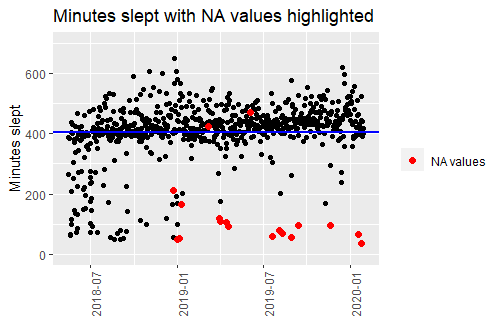
\includegraphics[width=1\linewidth]{https://i.ibb.co/nsFLV6z/naps} \caption{NA sleep values}\label{fig:na_sleep_values}
\end{figure}

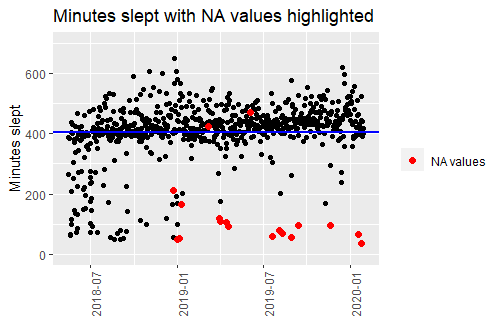
\includegraphics{./c73a3363277d31270c7c3c6fa489850fb4cfd40c.png}

This plot implicates that quite some of those values are rather short
sleep periods, possibly too short to get to different sleep phases. Most
of the individual \texttt{NA} values are significantly under der average
sleeptime.

\hypertarget{weekday-effect}{%
\subsubsection{Weekday Effect}\label{weekday-effect}}

Something that seems quite obvious is that behavior is not the same
throughout the week. One would expect longer sleep periods during
weekends and potentially irregular activity levels. Those might affect
calorie expenditure and amount of steps per weekday. I decided to check
on this hypothesis.

\begin{figure}
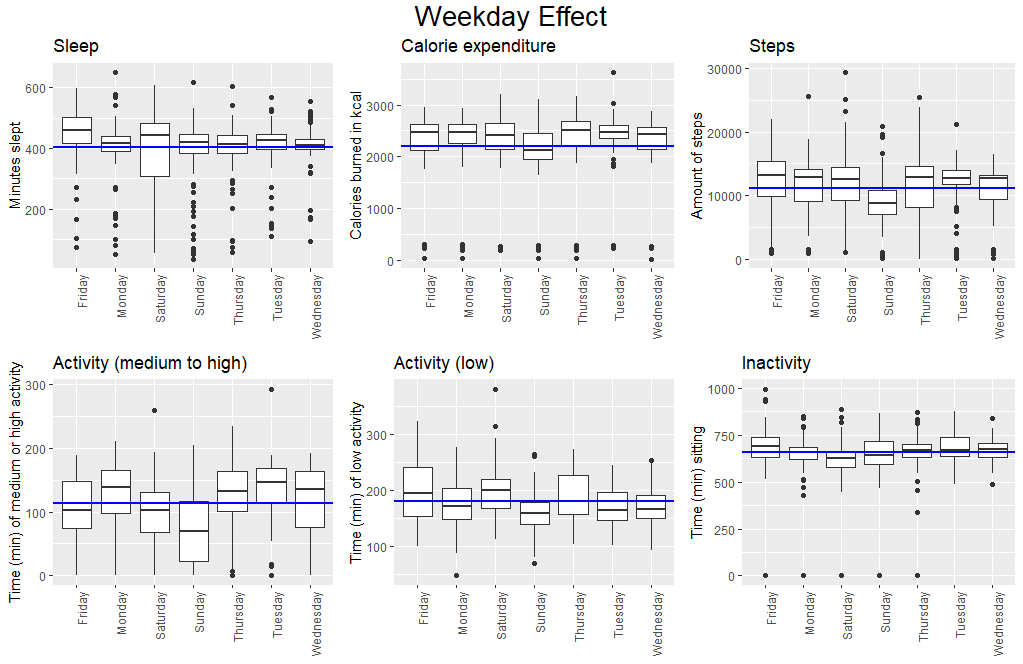
\includegraphics[width=1\linewidth]{Weekday_effect_fitbit} \caption{Weekday effect}\label{fig:weekday_effect}
\end{figure}

The blue lines in all plots of Figure \ref{fig:weekday_effect} indicate
the average value. For sleep, it becomes obvious that I sleep on average
longer on Fridays and Saturdays, whereas Saturday also has the biggest
interrange quartile (between approx 300 and 430 Minutes). In general,
the quartiles are all rather similar and rather small across the
weekdays.

When it comes to calorie expenditure, all days except for Sunday have a
median above average with a similarly small quartile and low
interquartile range.

For steps, the effect is slightly bigger even, with Sunday being below
average for the entire interquartile range. From the two plots, a
correlation between steps and calorie expenditure already seems
possible.

Medium to highly exhausting activity shows the biggest differences
between medians of individual weekdays with Friday and Saturday being
slightly under average and Sunday being clearly under average. The
interquartile range is bigger than in the three previous plots. Activity
that is in a lower heart frequency range (low activities) follows a
different trend: Monday, Saturday, Sunday, Tuesday, and Wednesday are
below average.

Hypothetically speaking, one could assume that on days with highly
demanding activities, the low activities might be decreased and
increased on days with less exhausting activities. Sunday is again the
only exception from this hypothesis and appears to be a day of rest for
me more often than not.

Inactivity, measured by minutes spent sitting, are across all weekdays
very similarly distributed with again a low interquartile range.

\hypertarget{sleep-details}{%
\subsubsection{Sleep Details}\label{sleep-details}}

In the Fitbit dataset, there is quite some level of detail for different
sleep phases. It appears obvious that activities might have an impact on
sleep quality and sleep duration. I decided to explore the data via some
plots around sleep details:

\begin{figure}
\centering
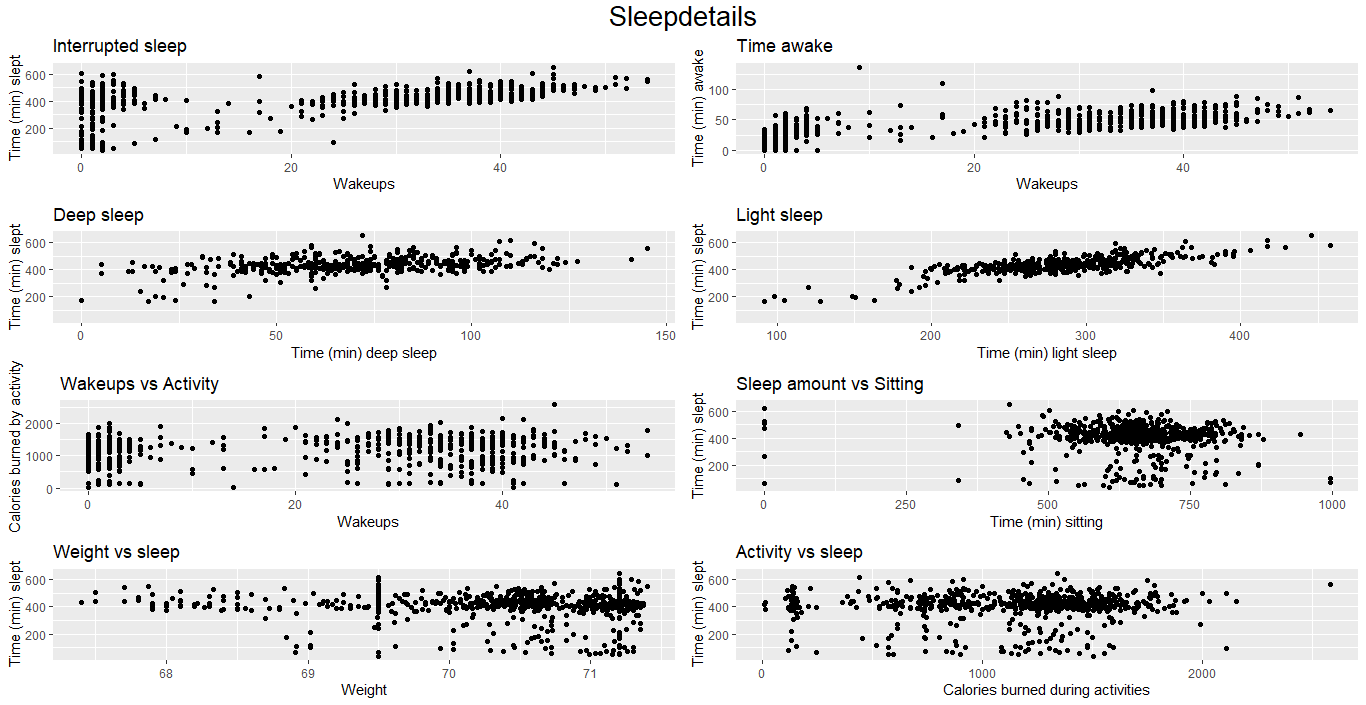
\includegraphics{./bf7a7a1effe1820d1bd6d9fb06c3ae37937c106b.png}
\caption{Sleepdetails}
\end{figure}

The first plot shows the correlation between overall time spent sleeping
and the number of times I woke up per night. As to be expected, with
higher sleep duration the number of wakeups tends to increase. We can
see a similar positive correlation between time awake (meaning time that
I was awake while I was in bed) and amount of wakeups.

The time spent in deep sleep appears to only slightly increase with an
increase in overall sleep time. The correlation between light sleep and
overall sleep time appears to be stronger.

There is no clear correlation between calories burned by activities
(indicating higher and lower activity levels per day) and the number of
wakeups. Similarly, there is also no clear correlation between
inactivity (minutes spent sitting) and overall time slept.

For the plot that indicates weight vs sleep time, it is visible that
many values were logged with the same weight (69.5 kg and slightly above
71 kg). Overall, significantly more values were logged for weight
\textgreater69 kg which is why it is tough to confirm any correlation.
We will see later in a regression tree that there appears to be at least
some indication from the weight value.

In the last plot, the relationship between activity level and overall
sleep amount is explored. It seems to be not correlated.

\hypertarget{regression-trees}{%
\subsubsection{Regression Trees}\label{regression-trees}}

After the data exploration via plots, a more holistic view on driving
factors for predictions was gathered for calorie expenditure, and sleep
data.

\hypertarget{calorie-expenditure}{%
\paragraph{Calorie Expenditure}\label{calorie-expenditure}}

For calorie expenditure, the full data set of \texttt{fitbit\_data} was
used, resulting in the following tree:

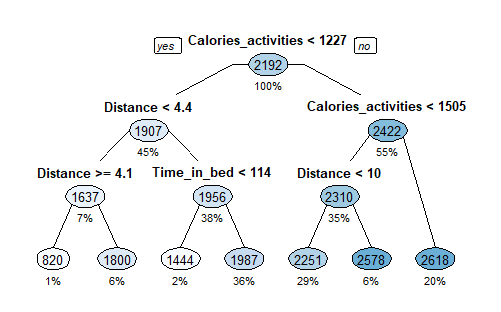
\includegraphics{./f7923d3e7bd7aaef585d684a7090278b230ea30d.png}

The main driver for the burned calories is the calories burned by sports
(calories\_activities). The value for differentiation is 1227 (kcal).
55\% of the data lies above that value, 20\% of the values even have a
value greater than 1505 (kcal). If the value is between 1227 and 1505,
Distance \textless{} 10 (in km) is the differentiating factor. Only 8\%
of the data is from days where the calories burned by sports were below
1505 (kcal) but the walked distance was above 10 (km).

Also on the other side of the tree, where the value for calories burned
by sports is below 1227 (kcal), the distance stays the next main driver
with a value of 4.4 (km) as a differentiator. For those occurrences
where the value is greater, time in bed is the next node in the tree,
with only 2\% being under the threshold of 114 (min) and 36\% of the
data being above it. For the occurrences where the value of 4.4 (km) was
not reached, the next node is again on distance for a slightly lower
value (4.1 (km)) as a differentiator that covers overall only 7\% of the
data.

\hypertarget{sleep}{%
\paragraph{Sleep}\label{sleep}}

For sleep duration, the data set of \texttt{fitbit\_data} still
contained data that would have been misleading: \texttt{Minutes\_awake},
\texttt{Minutes\_REM}, \texttt{Minutes\_light\_sleep},
\texttt{Minutes\_deep\_sleep}, \texttt{Wakeup\_amount} and
\texttt{Time\_in\_bed} all contain values that are directly related to
the overall sleep time and should not be included when e.g.~running
predictions.

Therefore, those columns are excluded first and the tree is built with
the data frame \texttt{fitbit\_data\_stripped}.

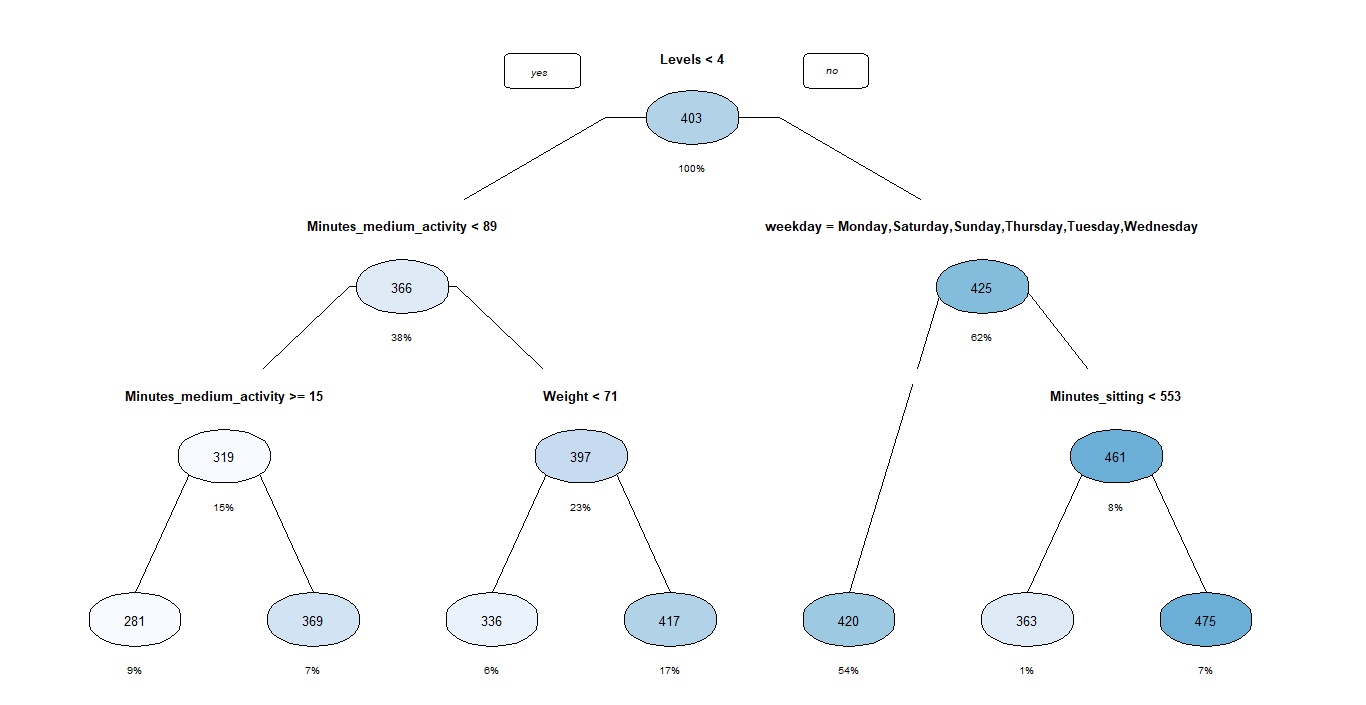
\includegraphics{./cd7f2afec0cdb99ee7abbf92e5e9d4e10143edc0.png}

The top of the tree is \texttt{Levels} which describes how many floors -
or how much altitude - were overcome at a given day. 62\% of the data
lay above a value of 4. For that 62 \%, the next determining factor is
indeed the Weekday: 54\% of the data goes directly to a leaf, explicitly
all weekdays except for Friday. For Friday, the only remaining node
differentiates by looking at the time spent sitting with a
differentiating value of 553 (minutes).

If on a given day, less than 4 levels had been overcome (38\%), minutes
in medium activity are evaluated next. If those are over 89 (minutes),
weight becomes a driving factor with a differentiating value of 71 (kg).
Otherwise, the time spent with medium activity is checked.

\hypertarget{data-prediction}{%
\subsection{Data Prediction}\label{data-prediction}}

To perform predictions, in general the function
\texttt{prediction(tolerance,\ testset,\ trainset,\ column,\ average,\ plottitle,\ xtitle,\ ytitle)}
is called. This function handles for all four predictions (Calories
Burned with NA excluded, Calories Burned with NA substituted by rnorm,
Calories Burned with NA substituted by mean and Sleep) by accepting all
needed values to handle those calculations. The function returns a plot
of the performance of the different models as well as the normalized
Root Mean Square Error (NRMSE). \texttt{tolerance} is a sequence of
numbers that defins a tolerated deviation from the predicted value.
\texttt{testset} is the test dataframe, \texttt{trainset} the training
dataframe and \texttt{column} marks the column that needs to be
evaluated. \texttt{average} is the respective average value to be used
for a very naive approach, that compares all models to predicting only
averages. \texttt{plottitle} sets the correct title for the output plot,
while \texttt{xtitle} and \texttt{ytitle} label the axis.

The call for e.g.~prediction of burned calories looks like this:

\begin{Shaded}
\begin{Highlighting}[]
\NormalTok{cal_tolerance<-}\KeywordTok{seq}\NormalTok{(}\DecValTok{0}\NormalTok{,}\DecValTok{100}\NormalTok{,}\DecValTok{10}\NormalTok{)}

\KeywordTok{prediction}\NormalTok{(cal_tolerance, fitbit_test, fitbit_train, }\StringTok{"Calories_Burned"}\NormalTok{,}
\NormalTok{           average_calories,}
           \StringTok{"Model performance for prediction of calorie expenditure"}\NormalTok{,}
           \StringTok{"+-Tolerance (in kcal)"}\NormalTok{, }\StringTok{"Performance of model"}\NormalTok{)}
\end{Highlighting}
\end{Shaded}

\hypertarget{calorie-expenditure-prediction}{%
\subsubsection{Calorie Expenditure
Prediction}\label{calorie-expenditure-prediction}}

For calorie expenditure, the entire dataset of \texttt{fitbit\_train} is
used to fit different models and predict on their basic values to
compare with \texttt{fitbit\_test}. Following, all model predictions
alongside a model that is only predicting the average value are
compared.

Since the values are so complex, an exact hit without any margin is
unlikely and a certain tolerance can and should be granted. For that
purpose, all predicted values are evaluated against whether their value
lies within tolerance.

In the following codeblock, the given column is put as a formula, that
can then be used for training. The fitted model is then used to predict
values on the testset.

\begin{Shaded}
\begin{Highlighting}[]
\NormalTok{  form <-}\StringTok{ }\KeywordTok{as.formula}\NormalTok{(}\KeywordTok{paste}\NormalTok{(column, }\StringTok{'~ .'}\NormalTok{))}
\NormalTok{    fitted <-}\StringTok{ }\KeywordTok{lapply}\NormalTok{(models, }\ControlFlowTok{function}\NormalTok{(model)\{ }
    \KeywordTok{print}\NormalTok{(model)}
    \KeywordTok{train}\NormalTok{(form, }\DataTypeTok{method =}\NormalTok{ model, }\DataTypeTok{data =}\NormalTok{ trainset, }\DataTypeTok{na.action=}\NormalTok{na.exclude)}
\NormalTok{  \}) }
  \KeywordTok{names}\NormalTok{(fitted) <-}\StringTok{ }\NormalTok{models}
\NormalTok{  prediction <-}\StringTok{ }\KeywordTok{sapply}\NormalTok{(fitted, }\ControlFlowTok{function}\NormalTok{(object) }
    \KeywordTok{predict}\NormalTok{(object, }\DataTypeTok{newdata =}\NormalTok{ testset, }\DataTypeTok{na.action=}\NormalTok{na.exclude))}
\end{Highlighting}
\end{Shaded}

The same prediction is repeated with the dataset
\texttt{fitbit\_train\_no\_na} and \texttt{fitbit\_train\_mean} that
contain no \texttt{NA} values.

\hypertarget{sleep-prediction}{%
\subsection{Sleep Prediction}\label{sleep-prediction}}

For sleep prediction, \texttt{fitbit\_train} was once more stripped from
overpredicting values as mentioned before and stored in this format
under \texttt{fitbit\_traindata\_stripped}. Following, all model
predictions alongside a model that is only predicting the average value
are compared. Since the values are complex an exact hit without any
margin is unlikely and a certain tolerance can and should be granted.
For that purpose, all predicted values are evaluated against whether
their value lies within tolerance.

\begin{Shaded}
\begin{Highlighting}[]
\CommentTok{#take out detailed data about sleep}
\NormalTok{fitbit_traindata_stripped <-}\StringTok{ }\NormalTok{fitbit_train }\OperatorTok
\StringTok{  }\KeywordTok{select}\NormalTok{(}\OperatorTok{-}\NormalTok{Minutes_awake, }\OperatorTok{-}\NormalTok{Minutes_REM, }
         \OperatorTok{-}\NormalTok{Minutes_light_sleep, }\OperatorTok{-}\NormalTok{Minutes_deep_sleep,}
         \OperatorTok{-}\NormalTok{Wakeup_amount, }\OperatorTok{-}\NormalTok{Time_in_bed, }\OperatorTok{-}\NormalTok{Date)}
\end{Highlighting}
\end{Shaded}

\newpage

\hypertarget{results}{%
\section{Results}\label{results}}

\hypertarget{calorie-expenditure-prediction-1}{%
\subsection{Calorie Expenditure
Prediction}\label{calorie-expenditure-prediction-1}}

The following plot shows the performance of all models for different
tolerance values \texttt{val\textless{}-seq(0,100,10)} from 0 to 100 in
steps of 10. This value is the tolerance granted for a hit below or
above the actual predicted value. In the case of tolerance of
\texttt{100}, this means that for a predicted value of \texttt{1800}
(kcal), an actual value of \texttt{1700} (kcal) or \texttt{1900}
respectively would lead to a hit. 100 kcal is approximately equivalent
to an apple or one glass (250 ml) of Coca Cola which I consider as an
acceptable deviation.

The plot also contains an ensemble-line that results from uniting all
models.

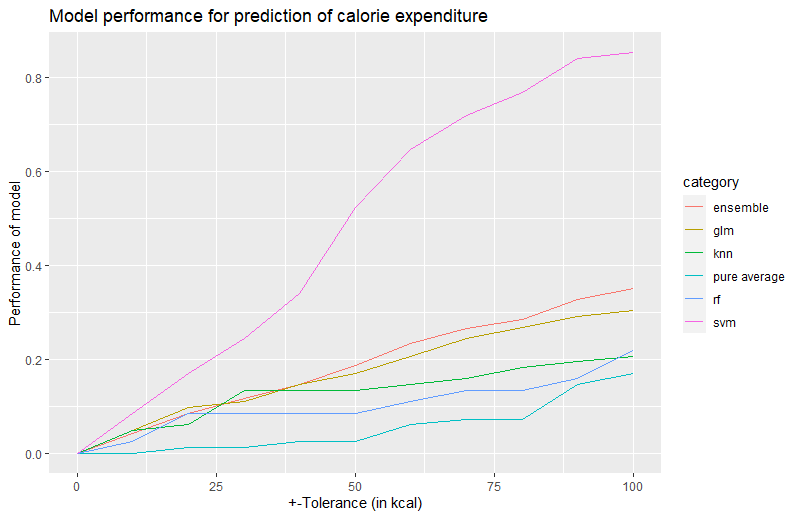
\includegraphics{./0b26bbe97576aac768e331f7c2dde9223408a268.png}

The graph shows that all models outperform the pure average. Logically,
all values increase with increasing tolerance, allowing to cover more
data range.

The SVM linear model by far outperforms other models and is correct with
a tolerance of 100 in approx. 85\% of the cases. Even the ensemble model
performs only on 35\% at the same tolerance value.

To evaluate Instead of Root Mean Square Error (RMSE), the Normalized
Root Mean Square Error (NRMSE) was used with
\(NRMSE=\frac{RMSE}{\bar{y}}\) where \(\bar{y}\) is the mean of the
actual values.

\begin{Shaded}
\begin{Highlighting}[]
\NormalTok{NRMSE <-}\StringTok{ }\ControlFlowTok{function}\NormalTok{(true_ratings, predicted_ratings)\{}
  \KeywordTok{sqrt}\NormalTok{(}\KeywordTok{mean}\NormalTok{((true_ratings }\OperatorTok{-}\StringTok{ }\NormalTok{predicted_ratings)}\OperatorTok{^}\DecValTok{2}\NormalTok{))}\OperatorTok{/}\KeywordTok{mean}\NormalTok{(true_ratings)}
\NormalTok{\}}
\end{Highlighting}
\end{Shaded}

The NRMSE confirms the plot: It is lowest with SVM Linear
(\texttt{svm}), followed by the General Linear Model (\texttt{glm}) and
K-nearest Neighbor (\texttt{knn}). The ensemble is not represented in
the table below.

\begin{Shaded}
\begin{Highlighting}[]
\OperatorTok{|}\NormalTok{method               }\OperatorTok{|}\StringTok{     }\NormalTok{NRMSE}\OperatorTok{|}
\ErrorTok{|:}\OperatorTok{--------------------}\ErrorTok{|}\OperatorTok{---------}\ErrorTok{:|}
\ErrorTok{|}\NormalTok{Random Forest        }\OperatorTok{|}\StringTok{ }\FloatTok{0.2587958}\OperatorTok{|}
\ErrorTok{|}\NormalTok{General Linear Model }\OperatorTok{|}\StringTok{ }\FloatTok{0.2477857}\OperatorTok{|}
\ErrorTok{|}\NormalTok{SVM Linear           }\OperatorTok{|}\StringTok{ }\FloatTok{0.2267550}\OperatorTok{|}
\ErrorTok{|}\NormalTok{K}\OperatorTok{-}\NormalTok{nearest Neighbor   }\OperatorTok{|}\StringTok{ }\FloatTok{0.2529889}\OperatorTok{|}
\ErrorTok{|}\NormalTok{Pure average         }\OperatorTok{|}\StringTok{ }\FloatTok{0.3060001}\OperatorTok{|}
\end{Highlighting}
\end{Shaded}

\hypertarget{dataset-without-nas-substituted-by-rnorm}{%
\subsubsection{Dataset without NA's substituted by
rnorm}\label{dataset-without-nas-substituted-by-rnorm}}

Originally, a separate dataset \texttt{fitbit\_train\_no\_na} was
created in the hope to improve predicitions by keeping datasets that
contain NA data in two to three columns. In the first prediction, those
were handled via \texttt{na.action=na.exclude} which concerned 294 rows.
The analysis shows that this had minimum impact on the performance of
all models.

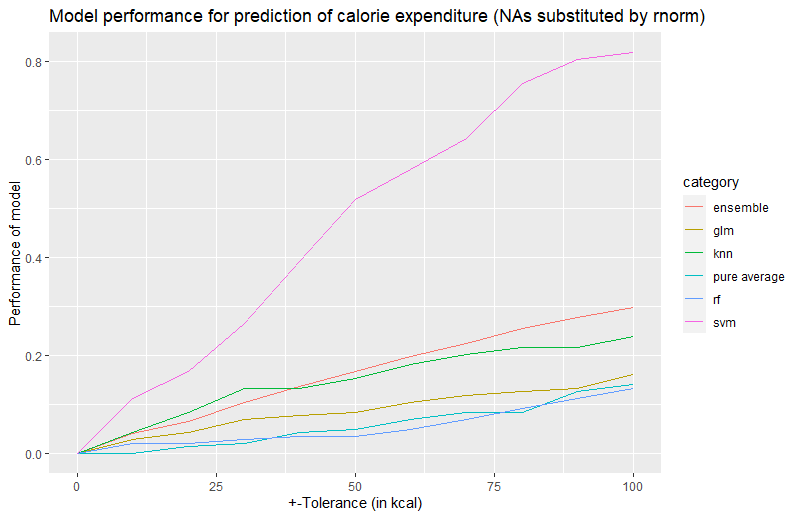
\includegraphics{./853f95ba287983e0cbab1a223bfd4b93b1858d68.png}

\begin{Shaded}
\begin{Highlighting}[]
\OperatorTok{|}\NormalTok{method               }\OperatorTok{|}\StringTok{     }\NormalTok{NRMSE}\OperatorTok{|}
\ErrorTok{|:}\OperatorTok{--------------------}\ErrorTok{|}\OperatorTok{---------}\ErrorTok{:|}
\ErrorTok{|}\NormalTok{Random Forest        }\OperatorTok{|}\StringTok{ }\FloatTok{0.3011162}\OperatorTok{|}
\ErrorTok{|}\NormalTok{General Linear Model }\OperatorTok{|}\StringTok{ }\FloatTok{0.2918140}\OperatorTok{|}
\ErrorTok{|}\NormalTok{SVM Linear           }\OperatorTok{|}\StringTok{ }\FloatTok{0.2750883}\OperatorTok{|}
\ErrorTok{|}\NormalTok{K}\OperatorTok{-}\NormalTok{nearest Neighbor   }\OperatorTok{|}\StringTok{ }\FloatTok{0.2949886}\OperatorTok{|}
\ErrorTok{|}\NormalTok{Pure average         }\OperatorTok{|}\StringTok{ }\FloatTok{0.3250873}\OperatorTok{|}
\end{Highlighting}
\end{Shaded}

The table show that the normalized mean square error has increased,
leading to lower accuracy of predictions.

Looking back at the data introduced via

\begin{Shaded}
\begin{Highlighting}[]
\KeywordTok{rnorm}\NormalTok{(}\DataTypeTok{n=}\KeywordTok{sum}\NormalTok{(}\KeywordTok{is.na}\NormalTok{(x)), }\DataTypeTok{mean=}\KeywordTok{mean}\NormalTok{(x, }\DataTypeTok{na.rm=}\OtherTok{TRUE}\NormalTok{),}\DataTypeTok{sd=}\KeywordTok{sd}\NormalTok{(x, }\DataTypeTok{na.rm=}\OtherTok{TRUE}\NormalTok{))}
\end{Highlighting}
\end{Shaded}

it becomes clear that some of the values are now negative, where they
really can't be.

\hypertarget{dataset-without-nas-substituted-by-mean}{%
\subsubsection{Dataset without NA's substituted by
mean}\label{dataset-without-nas-substituted-by-mean}}

Therefore, a new dataset was created after initial analysis in order to
check whether mean values would perform better as substitutes for NA
values.

Both, plot and NRMSE show that they actually do. The performance is
still slightly behin the model that completely ignores \texttt{NA}
values.

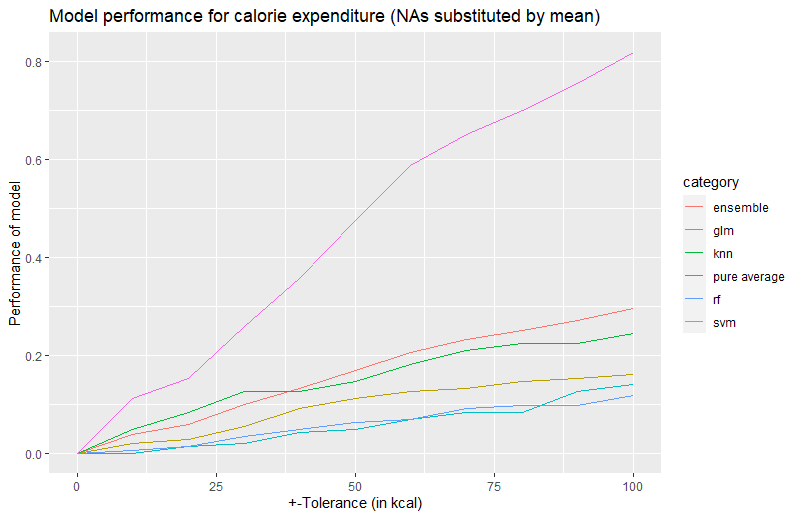
\includegraphics{./e26ac17ff62822ef527b8273128e2aae88d54615.png}

\begin{Shaded}
\begin{Highlighting}[]
\OperatorTok{|}\NormalTok{method               }\OperatorTok{|}\StringTok{     }\NormalTok{NRMSE}\OperatorTok{|}
\ErrorTok{|:}\OperatorTok{--------------------}\ErrorTok{|}\OperatorTok{---------}\ErrorTok{:|}
\ErrorTok{|}\NormalTok{Random Forest        }\OperatorTok{|}\StringTok{ }\FloatTok{0.2988310}\OperatorTok{|}
\ErrorTok{|}\NormalTok{General Linear Model }\OperatorTok{|}\StringTok{ }\FloatTok{0.2972105}\OperatorTok{|}
\ErrorTok{|}\NormalTok{SVM Linear           }\OperatorTok{|}\StringTok{ }\FloatTok{0.2754964}\OperatorTok{|}
\ErrorTok{|}\NormalTok{K}\OperatorTok{-}\NormalTok{nearest Neighbor   }\OperatorTok{|}\StringTok{ }\FloatTok{0.2905055}\OperatorTok{|}
\ErrorTok{|}\NormalTok{Pure average         }\OperatorTok{|}\StringTok{ }\FloatTok{0.3250873}\OperatorTok{|}
\end{Highlighting}
\end{Shaded}

\hypertarget{sleep-prediction-1}{%
\subsection{Sleep Prediction}\label{sleep-prediction-1}}

The following plot shows the performance of all models for different
tolerance values \texttt{val\_sleep\textless{}-seq(0,30,2)} from 0 to 30
in steps of 2. This value is the tolerance granted for a hit below or
above the actual predicted value. In the case of tolerance of
\texttt{30}, this means that for a predicted value of \texttt{400}
(min), an actual value of \texttt{330} (min) up to a value of
\texttt{430}(min) would lead to a hit.

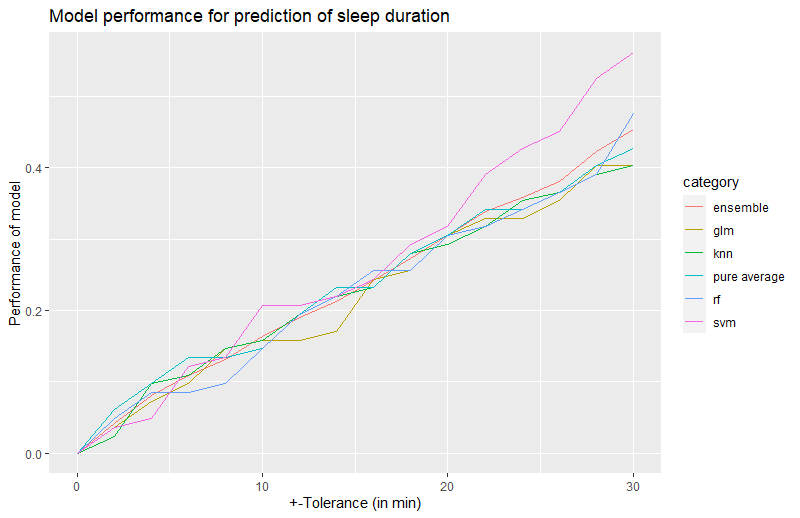
\includegraphics{./4c54cac10838a095c48f2a179f2d9d8f708daa17.png}

The graph shows that most models barely outperform the pure average.
Logically, all values increase with increasing tolerance, allowing to
cover more data range. The SVM linear model slightly outperforms other
models and is correct with a tolerance of 30 in only approx. 56\% of the
cases.

To evaluate Instead of Root Mean Square Error (RMSE), the Normalized
Root Mean Square Error (NRMSE) was used with
\(NRMSE=\frac{RMSE}{\bar{y}}\) where \(\bar{y}\) is the mean of the
actual values.

\begin{Shaded}
\begin{Highlighting}[]
\NormalTok{NRMSE <-}\StringTok{ }\ControlFlowTok{function}\NormalTok{(true_ratings, predicted_ratings)\{}
  \KeywordTok{sqrt}\NormalTok{(}\KeywordTok{mean}\NormalTok{((true_ratings }\OperatorTok{-}\StringTok{ }\NormalTok{predicted_ratings)}\OperatorTok{^}\DecValTok{2}\NormalTok{))}\OperatorTok{/}\KeywordTok{mean}\NormalTok{(true_ratings)}
\NormalTok{\}}
\end{Highlighting}
\end{Shaded}

The NRMSE confirms the plot: It is lowest with SVM Linear
(\texttt{svm}), followed by the Random Forest Model (\texttt{rf}) and
General Linear Model (\texttt{glm}). The ensemble is not represented in
the table below.

\begin{Shaded}
\begin{Highlighting}[]
\OperatorTok{|}\NormalTok{method               }\OperatorTok{|}\StringTok{     }\NormalTok{NRMSE}\OperatorTok{|}
\ErrorTok{|:}\OperatorTok{--------------------}\ErrorTok{|}\OperatorTok{---------}\ErrorTok{:|}
\ErrorTok{|}\NormalTok{Random Forest        }\OperatorTok{|}\StringTok{ }\FloatTok{0.1629523}\OperatorTok{|}
\ErrorTok{|}\NormalTok{General Linear Model }\OperatorTok{|}\StringTok{ }\FloatTok{0.1842242}\OperatorTok{|}
\ErrorTok{|}\NormalTok{SVM Linear           }\OperatorTok{|}\StringTok{ }\FloatTok{0.1659489}\OperatorTok{|}
\ErrorTok{|}\NormalTok{K}\OperatorTok{-}\NormalTok{nearest Neighbor   }\OperatorTok{|}\StringTok{ }\FloatTok{0.1926286}\OperatorTok{|}
\ErrorTok{|}\NormalTok{Pure average         }\OperatorTok{|}\StringTok{ }\FloatTok{0.1707393}\OperatorTok{|}
\end{Highlighting}
\end{Shaded}

\newpage

\hypertarget{conclusion}{%
\section{Conclusion}\label{conclusion}}

Starting with the assumption that sleep patterns and calorie expenditure
are based on weekdays and activity throughout the day, I can only
partially confirm my assumption based on the data collected over the
course of over 2.5 years.

While there is a good chance to predict calorie expenditure based on
activity data, the prediction of sleep is unsatisfactory.

For this assessment, I have not used all of the data that I can gather
from Fitbit. Blood oxygen saturation values can be retrieved and can
indicate recovery, and could, therefore, improve sleep prediction
accuracy. Also, heart rate can be exported which might be equally
relevant and could also further improve calorie expenditure prediction.

Quite surprising to me was the impact of \texttt{NA} value handling that
I did not expect.

\end{document}
